\documentclass[twoside]{hcmut-report}

\begin{document}
\fancyfoot{}
\coverpage\clearpage

\pagenumbering{Roman}
\fancyfoot[C]{
	\ttfamily
	\thepage
}
\part*{Declaration} \label{part:declaration}
We, the undersigned -- Doan Phuong Hung Cuong, Nguyen Thien Hao, and Pham Quang Hieu -- hereby submit this Specialized Project Report, titled \textit{``An End-to-End \acs{MLOps} Pipeline for Cross-Sectional Equity Ranking under Data Constraints: Engineering Validation and Ablation Study''}, in partial fulfillment of the academic requirements. We solemnly declare that this manuscript represents the authentic outcome of our independent research, system architecture design, and empirical validation, conducted under the supervision of {\color{red}Dr. Pham An Vinh} and {\color{red}Dr. Nguyen An Khuong}.

We explicitly affirm the following statements regarding academic integrity, ethical standards, and original authorship:
\begin{itemize}[topsep=0pt, itemsep=0pt, parsep=0pt]
	\item \textbf{Originality and Intellectual Attribution:} All methodologies, algorithms, data sources, and literature referenced herein that are not our original creation have been explicitly acknowledged, formally cited, and referenced in strict compliance with established academic standards.
	\item \textbf{Code Ownership and Reproducibility:} All software artifacts, system architectures, and codebase implementations were engineered by the authors. Any third-party libraries, open-source frameworks, or cloud infrastructures utilized within the pipeline have been properly cited and applied in accordance with their respective licenses.
	\item \textbf{Disclosure of \acs{AI} and \acs{LLMs} Assistance:} Generative \ac{AI} systems and \ac{LLMs} were utilized strictly as supportive tools for syntactic refinement, prose editing, and structural organization. No core technical architectures, empirical analyses, feature engineering logic, or conclusions were synthesized by automated tools. The authors retain full ownership of and accountability for all intellectual content.
	\item \textbf{Data Integrity and Empirical Veracity:} All computational experiments, performance metrics, and ablation outcomes presented in this work reflect genuine implementation results without fabrication, falsification, or deliberate omission of data.
	\item \textbf{Exclusivity of Submission:} This research work is original and has not been submitted, either in whole or in part, for the award of any other academic degree, diploma, or professional qualification at this or any other institution.
\end{itemize}

\begin{flushright}
	\textit{Ho Chi Minh City, \today}
\end{flushright}

\vspace{3cm}

\noindent
\begin{minipage}{0.35\textwidth}
	\centering
	\hrulefill \\
	\vspace{0.2cm}
	\textbf{Doan Phuong Hung Cuong}
\end{minipage}
\hfill
\begin{minipage}{0.3\textwidth}
	\centering
	\hrulefill \\
	\vspace{0.2cm}
	\textbf{Nguyen Thien Hao}
\end{minipage}
\hfill
\begin{minipage}{0.3\textwidth}
	\centering
	\hrulefill \\
	\vspace{0.2cm}
	\textbf{Pham Quang Hieu}
\end{minipage}
\clearpage

\part*{Acknowledgment} \label{part:acknowledgment}
First and foremost, we extend our deepest gratitude to \textcolor{red}{Dr. Pham An Vinh} for his outstanding technical mentorship and visionary guidance throughout this project. His expertise in quantitative finance and practical insights into alpha strategies were central to our research. His real-world experience helped us address the complexities of modeling financial markets, recognizing statistical trends, and analyzing microstructure dynamics. Moreover, his rigorous supervision greatly enhanced the precision of our quantitative analysis, including empirical evaluation, feature engineering, and backtesting of our equity ranking pipelines.

\medskip

We also wish to express our sincere appreciation to our supervisor, \textcolor{red}{Dr. Nguyen An Khuong}. His invaluable support and steadfast academic guidance have been instrumental in refining our technical acumen and instilling a rigorous, systematic approach to both our research and engineering efforts. We are especially thankful for his generous provision of foundational academic materials and specialized literature, which proved critical to the successful formulation, structural organization, and execution of our research objectives.

\medskip

We also extend our earnest appreciation to \textcolor{red}{Mr. Nguyen Duong Nhat} (M.Sc. Candidate, \href{https://www.fau.de/}{FAU}) and \textcolor{red}{Miss Truong Nguyen Duyen Anh} (B.A. Candidate, \href{https://www.uni-augsburg.de/en/}{Universität Augsburg}) for their invaluable assistance in sourcing and compiling the datasets utilized in this thesis. Additionally, we are deeply grateful to \textcolor{red}{Mr. Nguyen Khac Khanh Huy} (B.A. Candidate, \href{https://hcmut.edu.vn/}{HCMUT}) for his vital contributions in engineering and constructing the robust data warehouse infrastructure. Their collective efforts in data acquisition, preparation, and architectural design provided the essential technical foundation for the empirical analysis and validation of our quantitative models.

\medskip

Our sincere thanks are directed to the Faculty of Computer Science and Engineering at \href{https://hcmut.edu.vn}{\textcolor{blue}{Ho Chi Minh City University of Technology} \inlinelogo{images/hcmut-logo.png}} for fostering a stimulating academic environment and supplying the foundational resources requisite for conducting this specialized study.

\medskip

Furthermore, we gratefully acknowledge \href{https://modal.com}{\textcolor{modal-color}{Modal} \inlinelogo{images/modal-logo.png}} for their generous provision of cloud computing infrastructure. Access to their high-performance, complimentary \acl{GPU} resources was pivotal in overcoming our local hardware limitations, enabling the efficient execution of complex computational experiments, large-scale ablation studies, and the training of our machine learning pipelines.

\medskip

We also wish to recognize our peers and colleagues whose intellectual camaraderie, constructive feedback, and steadfast encouragement provided much-needed motivation during the more demanding phases of this project.

\medskip

Finally, we are eternally grateful to our families for their unwavering emotional support, patience, and understanding throughout the extensive development, implementation, and writing of this report.

\clearpage

\part*{Abstract}
% To be updated
\clearpage

\clearpage

\tableofcontents
\clearpage

\listoffigures
\listoftables
\part*{List of Abbreviations}
\begin{acronym}
	\acro{AI}{Artificial Intelligence}
	\acro{API}{Application Programming Interface}
	% \acro{CUDA}{Compute Unified Device Architecture}
	\acro{DSMA}{Distance from Simple Moving Average}
	% \acro{GICS}{Global Industry Classification Standard}
	\acro{GPU}{Graphics Processing Unit}
	\acro{IC}{Information Coefficient}
	\acro{ICIR}{Information Coefficient Information Ratio}
	\acro{LLMs}{Large Language Models}
	\acro{LSTM}{Long Short-Term Memory}
	\acro{MLOps}{Machine Learning Operations}
	\acro{NYSE}{New York Stocks Exchange}
	% \acro{SHAP}{SHapley Additive exPlanations}
	\acro{OHLCV}{Open-High-Low-Close-Volume}
	\acro{PVT}{Price Volume Trend}
	\acro{RSI}{Relative Strength Index}
	% \acro{SnP}[S\&P]{Standard \& Poor's}
	% \acro{XAI}{Explainable Artificial Intelligence}
\end{acronym}
\clearpage

\pagenumbering{arabic}
\setcounter{page}{1}
\fancyfoot{} % Remove Roman page counter
\startfooter{Specialized Project: HK261-DAGD1-041\\
	Introduction
}

\part{Introduction} \label{part:introduction}

\section{Context and Motivation} \label{sec:context-and-motivation}
Machine learning has become an increasingly important methodological tool in quantitative finance because of its ability to model nonlinear relationships and interactions among large sets of financial predictors. In a large-scale empirical study of equity returns, Gu, Kelly, and Xiu~\cite{Gu2020} show that machine learning methods can improve return forecasting relative to conventional linear approaches, with part of the predictive improvement arising from nonlinear interactions among characteristics. Their results also identify momentum, liquidity, and volatility-related variables among the dominant predictors of expected returns. This evidence motivates the use of flexible nonlinear models when the objective is to extract information from a rich set of financial signals.

\medskip

Sequence-based deep learning models provide one approach to capturing temporal structure in financial data. Fischer and Krauss~\cite{FischerKrauss2018} demonstrate the application of \acf{LSTM} networks to financial market prediction and report that \acs{LSTM} models can exploit patterns in sequential stock data that are difficult to capture using simpler predictive models. More generally, the Transformer architecture~\cite{Vaswani2017} provides a mechanism for modeling relationships through attention, allowing a model to selectively incorporate information from multiple elements of an input sequence. These characteristics make recurrent and attention-based architectures potentially suitable for financial problems in which relevant information may be distributed across time and across simultaneously observed securities.

\medskip

The present study focuses specifically on the latter dimension. The objective is not to forecast the return of an individual stock in isolation, but to generate a \emph{cross-sectional ranking} of securities at each decision point. This distinction is fundamental because the economic decision in a cross-sectional strategy is based on the relative ordering of securities rather than the numerical accuracy of an isolated return forecast. Poh et al.~\cite{Poh2021} formalize this perspective and show that ranking-oriented learning methods can improve cross-sectional systematic strategies by directly learning pairwise and listwise relationships among instruments. The ranking problem therefore requires a modeling framework that preserves information about the contemporaneous cross-section instead of treating each security as an independent forecasting task.

\medskip

The cross-sectional nature of equity returns is also well established in the asset-pricing literature. Fama and French~\cite{FamaFrench1992} show that firm characteristics such as size and book-to-market equity are related to systematic differences in average stock returns, while Fama and French~\cite{FamaFrench1993} demonstrate that common risk factors account for substantial shared variation in stock returns. These findings motivate a distinction between systematic variation shared across securities and residual variation that may contain additional information about relative performance. In the present study, this distinction is reflected in the construction of a forward-return target that is residualized against common risk factors before cross-sectional evaluation.

\medskip

% The \acf{SnP} 500 is used as the empirical market universe because it provides a large and economically coherent cross-section of large-cap U.S. equities within which this relative-ranking problem can be studied. Fortune~\cite{Fortune1998} discusses the S\&P 500 as a benchmark portfolio intended to represent a particular segment of the U.S. equity market, while Cremers, Petajisto, and Zitzewitz~\cite{Cremers2013} explicitly examine the S\&P 500 as a passive benchmark in the evaluation of portfolio performance. The S\&P 500 is therefore treated in this study not as a representation of the entire U.S. equity market, but as a defined large-cap universe in which securities share broad market exposure while retaining meaningful cross-sectional differences.

% \medskip

% This distinction is particularly relevant because empirical research demonstrates that S\&P 500 constituents exhibit substantial variation in their systematic risk and market behavior. Andersen, Thyrsgaard, and Todorov~\cite{Andersen2021}, for example, document significant time variation in the cross-sectional dispersion of systematic risk among S\&P 500 constituents. Similarly, Hallin et al.~\cite{Hallin2011} show that liquidity measures across S\&P 500 constituents exhibit common dynamic factors, while Hegde and McDermott~\cite{Hegde2003} document changes in liquidity associated with S\&P 500 index membership. These findings support the use of the universe as a structured cross-section in which both common and security-specific information can be examined.

% \medskip

The research problem is therefore not simply to determine whether a flexible model can predict future stock returns. Rather, it is to determine whether temporal information and cross-sectional relationships can be combined to improve the ranking of securities within a common market universe. The proposed architecture addresses this problem by combining an \acs{LSTM}-based temporal encoder with a cross-sectional Transformer, allowing information about the historical evolution of an individual security to be processed jointly with information from the contemporaneous cross-section.

\section{Research Problem} \label{sec:research-problem}
The central research problem addressed in this thesis is the design and empirical validation of an end-to-end machine learning pipeline for cross-sectional equity ranking under the statistical, data, and implementation constraints inherent in financial markets.

\medskip

A conventional pointwise forecasting formulation assigns a prediction problem to each security separately. However, the investment decision considered in this study is inherently comparative: securities are ranked relative to their peers and subsequently incorporated into a portfolio according to their predicted relative performance. The learning objective must therefore reflect the structure of the downstream decision problem. This motivates the use of a ranking-aware learning objective in addition to the conventional regression objective, following the cross-sectional learning-to-rank perspective of Poh et al.~\cite{Poh2021}.

\medskip

At the same time, the predictive problem must account for common systematic variation. Because securities in the same market universe are exposed to shared market conditions, raw forward returns contain variation that may not represent security-specific information. The empirical design therefore residualizes the forward return against common factors before evaluating cross-sectional predictive performance. This approach is consistent with the role of common risk factors established in the asset-pricing literature~\cite{FamaFrench1992,FamaFrench1993}.

\medskip

A second dimension of the research problem concerns empirical validation. Financial observations are temporally ordered and may contain overlapping information across adjacent observations. Consequently, model evaluation must preserve chronological structure and distinguish information available at the prediction date from information that becomes available subsequently. Tashman~\cite{Tashman2000} emphasizes the importance of carefully designed out-of-sample evaluation and rolling-origin procedures in forecasting applications. In addition, extensive hyperparameter experimentation creates a multiple-testing problem: a model selected because it performs well over many trials may exhibit an inflated backtest performance even when the underlying strategy contains little genuine predictive information. Bailey and López de Prado~\cite{BaileyLopezDePrado2014} develop the Deflated Sharpe Ratio specifically to address selection bias and backtest overfitting arising from multiple testing.

\medskip

The research therefore treats validation as part of the model itself rather than as a separate reporting step. The proposed pipeline incorporates chronological walk-forward evaluation, purging and embargoing of observations around test periods, and explicit adjustment for multiple-testing effects. These procedures are intended to reduce the possibility that apparent predictive performance results from information leakage or repeated experimentation rather than from generalizable structure.

\medskip

Finally, the research considers the transition from statistical prediction to portfolio construction. A cross-sectional ranking may contain predictive information without being directly implementable as a portfolio. Portfolio decisions are affected by covariance estimation, position constraints, turnover, transaction costs, and market impact. The framework consequently evaluates the model's out-of-sample predictions within a constrained portfolio construction process. The importance of accounting for execution costs and market impact in portfolio implementation is established in the optimal-execution literature~\cite{AlmgrenChriss2000}.

\section{Research Gap} \label{sec:research-gap}
The first research gap concerns the alignment between prediction objectives and cross-sectional portfolio decisions. Standard regression-based forecasting evaluates the accuracy of individual return predictions, whereas cross-sectional strategies ultimately depend on the relative ranking of securities. Poh et al.~\cite{Poh2021} demonstrate the importance of learning the ranking structure directly. The present study extends this perspective by investigating a hybrid learning objective that combines pointwise prediction with pairwise ranking information within a deep temporal--cross-sectional architecture.

\medskip

The second gap concerns the integration of temporal and cross-sectional information within a single predictive framework. LSTM-based models provide a mechanism for learning sequential dependencies~\cite{FischerKrauss2018}, while attention-based models provide a mechanism for representing interactions among elements of an input set~\cite{Vaswani2017}. Existing empirical work establishes the usefulness of both nonlinear machine learning and cross-sectional structure in equity prediction~\cite{Gu2020,Poh2021}; however, the present study focuses on an integrated architecture in which temporal representations of individual securities are subsequently processed jointly across the cross-section.

\medskip

The third gap concerns validation under realistic financial data constraints. Machine learning models provide substantial flexibility, but that flexibility also increases exposure to data leakage, selection bias, and backtest overfitting. Tashman~\cite{Tashman2000} establishes the importance of carefully designed out-of-sample forecasting procedures, while Bailey and López de Prado~\cite{BaileyLopezDePrado2014} show that multiple testing can materially inflate apparent strategy performance. The present research incorporates these concerns directly into the experimental design through purged walk-forward validation, embargoing, and multiple-testing diagnostics.

\medskip

The fourth gap concerns the connection between predictive signals and implementable portfolios. Rather than evaluating the model solely through prediction accuracy, the study carries locked out-of-sample predictions into a constrained portfolio construction stage. This allows the robustness of the predictive signal to be examined after accounting for covariance risk and explicit transaction-cost and market-impact assumptions, consistent with the principles of optimal execution~\cite{AlmgrenChriss2000}.

\section{Research Questions} \label{sec:research-questions}
The central research question is:
\begin{quote}
	\textit{Can an end-to-end MLOps pipeline successfully engineer, validate, and constrain a hybrid temporal-attention (\acs{LSTM}--Transformer) architecture for cross-sectional equity ranking, and accurately translate its out-of-sample predictions into a strictly risk-neutralized portfolio under rigid computational and data constraints?}
\end{quote}

This question is investigated through two groups of research questions. The first concerns signal generation and model validation. It examines whether a hybrid loss combining Mean Squared Error (MSE) with a pairwise hinge loss improves the separation of predicted cross-sectional deciles relative to a pure pointwise objective, and whether a learned static Stock ID embedding contributes information beyond the temporal and cross-sectional market structure.

\medskip

The second group concerns portfolio construction and robustness. It examines the degradation of model-derived portfolio performance after the introduction of covariance risk and transaction costs, and evaluates the extent to which multiple-testing adjustment reduces the apparent performance obtained during model and hyperparameter selection.

\section{Research Contributions} \label{sec:research-contributions}
The contribution of this thesis is primarily methodological and empirical. It develops and evaluates an end-to-end framework for cross-sectional equity ranking in which predictive modeling, statistical validation, and portfolio construction are treated as interconnected components.

\medskip

\begin{itemize}[leftmargin=2.2cm, topsep=0pt, parsep=0pt]
	\item[\textit{First},] The study formulates the equity prediction problem explicitly as a cross-sectional ranking task rather than as a set of independent point forecasts.
	\item[\textit{Second},] It combines temporal representation learning through an \acs{LSTM} with cross-sectional attention through a Transformer, thereby allowing both within-security dynamics and contemporaneous inter-security relationships to be modeled.
	\item[\textit{Third},] It incorporates a ranking-aware training objective intended to align the optimization problem with the downstream portfolio decision.
	\item[\textit{Fourth},] The framework embeds chronological and leakage-aware validation procedures together with explicit control for multiple-testing bias.
	\item[\textit{Finally},] It evaluates the persistence of the generated signal after portfolio construction under covariance, leverage, position, turnover, and transaction-cost constraints.
\end{itemize}

\medskip

The study is deliberately framed as an engineering validation and empirical evaluation rather than a claim that the resulting model constitutes universally deployable trading alpha. The empirical analysis is conducted within the explicitly defined S\&P 500 research universe and its filtered analytical sample, and the methodological limitations associated with the available data are retained and discussed explicitly.

\section{Thesis Organization} \label{sec:thesis-organization}
The remainder of the thesis follows the sequence of the empirical pipeline. The methodology first defines the market universe and constructs the analytical sample, including the associated survivorship and classification considerations. The data-processing stage then describes the construction and transformation of the input variables and prediction target. The predictive modeling stage presents the temporal and cross-sectional architecture, the ranking-aware learning objective, and the experimental design. The subsequent evaluation examines predictive performance, statistical significance, model stability, and sensitivity to alternative specifications. Finally, the locked out-of-sample predictions are passed to the portfolio-construction framework, where the economic consequences of risk controls and transaction costs are evaluated before the methodological limitations and conclusions are presented.

\section{Overall Structure} \label{sec:overall-structure}
To be updated
\clearpage
% \setcounter{page}{1}
\startfooter{Specialized Project: HK261-DAGD1-041\\
    Thesis Proposal
}

\part{Thesis Proposal}

\section{Introduction}

\subsection*{Context and Motivation}

Deep learning architectures show immense theoretical promise in equity forecasting. Models such as \ac{LSTM} and Transformers can effectively capture nonlinear structures and complex dependencies embedded in financial time series, increasingly outperforming shallow machine learning models in asset return prediction~\cite{Ellery2025}. However, transitioning these highly parameterized models from theoretical environments to deployable pipelines requires robust \ac{MLOps} frameworks, ranking-aware objectives, and strict validation protocols.

\medskip

The current intersection of deep learning and quantitative finance faces a severe deployment gap. While academic literature frequently demonstrates superior theoretical precision in capturing temporal dependencies, real-world alpha generation requires modeling continuous cross-sectional dynamics rather than isolated time series. Furthermore, the true engineering challenge lies not in architectural complexity, but in strictly controlling for data constraints, mitigating data leakage, and constructing resilient pipelines capable of interacting with live convex optimization engines. Building this infrastructure under strict computational constraints is a critical engineering requirement.

\subsection*{Research Gaps}

\textbf{Gap 1 -- The disconnection between pointwise forecasting and ranking-aware portfolio construction.} The vast majority of deep learning financial forecasting models optimize pointwise losses (such as Mean Squared Error), treating each asset's return prediction independently. However, cross-sectional strategies generate alpha by trading assets against each other -- buying the top decile and selling the bottom decile. As demonstrated by Poh et al.~\cite{Poh2020}, utilizing Learning-to-Rank (LTR) algorithms and pairwise losses over pointwise losses substantially improves the trading performance of cross-sectional strategies by capturing the relational listwise structure of the instruments. Despite this, there is a lack of end-to-end \acs{MLOps} architectures that natively integrate hybrid ranking loss formulations (e.g., combining MSE with pairwise hinge loss) directly inside strict walk-forward validation loops.
\label{gap_1}

\bigskip

\textbf{Gap 2 -- Engineering validation under data constraints and multiple-testing bias.} Much of the existing literature abstracts away the mechanical friction of the market, assuming frictionless execution and perfect point-in-time data. Furthermore, the advent of high-performance computing allows analysts to test millions of hyperparameter configurations, inevitably leading to backtest overfitting. As established by Bailey and L\'opez de Prado~\cite{BaileyLopezdePrado2014}, failing to control for the number of trials leads to overly optimistic performance expectations. There is a critical engineering need for pipelines that natively default to deflated statistical metrics (such as the Deflated Sharpe Ratio) to strictly separate legitimate algorithmic edges from statistical flukes generated by hyperparameter optimization sweeps.
\label{gap_2}

\subsection*{Research Questions}
\textbf{Central Research Question:}\\
Can an end-to-end \acs{MLOps} pipeline successfully engineer, validate, and constrain a hybrid temporal-attention (LSTM-Transformer) architecture for cross-sectional equity ranking, and accurately translate its out-of-sample predictions into a strictly risk-neutralized portfolio under rigid computational and data constraints?

\medskip

\textbf{Phase 1 Research Questions (Signal Generation and \acs{MLOps} Validation):}
\begin{itemize}
    \item RQ1.1: How does a hybrid AlphaLoss formulation -- combining standard MSE with a pairwise hinge loss penalizing rank inversions -- improve the monotonic separation of predicted deciles compared to a pure pointwise MSE objective?
    \item RQ1.2: What is the quantitative impact of concatenating a learned 32-dimensional static Stock ID embedding to the LSTM's hidden state prior to the cross-sectional Transformer encoder, and does this specific ablation indicate structural survivorship-universe memorization?
\end{itemize}

\textbf{Phase 2 Research Questions (Constrained Portfolio Construction and Analytics):}
\begin{itemize}
    \item RQ2.1: When transitioning from raw signals to a convex optimization engine utilizing Ledoit-Wolf covariance shrinkage, how much do modeled transaction costs (integrating both a linear spread term and a quadratic market impact term) degrade the idealized portfolio performance?
    \item RQ2.2: Following an expanding 5-fold Purged Walk-Forward evaluation regime, to what degree does the application of the Deflated Sharpe Ratio mathematically reduce the perceived out-of-sample performance by strictly controlling for the multiple-testing bias inherent in the Optuna optimization sweeps?
\end{itemize}

\subsection*{Scope and Limitations}

\begin{itemize}
    \item \textbf{Data Universe Constraints:} The analysis is strictly constrained to the intersection of 413 \ac{SnP} 500 equities possessing complete, continuous daily split- and dividend-adjusted \ac{OHLCV} history from 2020-01-01 onward.
    \item \textbf{Structural Bias Acknowledgment:} No attempt is made to reconstruct delisted or merged names; therefore, a structural survivorship bias is present and explicitly acknowledged. Additionally, sector definitions rely on static, current \ac{GICS} Level 1 assignments, acting as an acknowledged approximation.
    \item \textbf{Leakage Prevention:} Intra-series missing bars or trading suspensions are strictly forward-filled to prevent look-ahead bias.
    \item \textbf{Nature of Results:} All financial metrics serve solely to validate mechanical pipeline health and must not be interpreted as deployable alpha.
    \item \textbf{System Validation vs. Inferential Claims:} The pipeline will be deployed to a brokerage \ac{API} for engineering validation (paper trading); however, these paper trading results are entirely excluded from financial conclusions, acting solely as validation of order routing and system orchestration.
    \item \textbf{Decoupled Architecture:} The data layer is intentionally decoupled; this design ensures that a survivorship-free point-in-time database can be substituted in the future without altering the core pipeline code.
\end{itemize}

\section{Specialized Project}
\subsection*{Decription:}
Phase 1 builds the core predictive layer of the entire system: an end-to-end \acs{MLOps} pipeline that transforms raw \acs{OHLCV} time series and factor data into strictly validated cross-sectional equity rankings. The architectural principle throughout is to enforce rigorous chronological integrity; the data layer is completely decoupled, ensuring strict forward-filling of intra-series missing bars to prevent look-ahead bias. The pipeline is organized into five functional layers:
\begin{enumerate}
    \item \textbf{Target Residualization \& Cross-Sectional Z-Scoring:} Extracts a 5-day forward excess return residualized against a multi-factor risk model (Fama-French Market, SMB, HML, and Volatility factors) to isolate asset-specific price-volume dynamics. According to Fama and French~\cite{FamaFrench1993}, extracting common risk factor exposures is necessary to isolate true idiosyncratic returns (alpha) from systematic market betas.
    \item \textbf{Tensor Construction:} Formulates structured temporal-cross-sectional input tensors of shape $[\text{Batch\_Dates}, 413, 60, 15]$.
    \item \textbf{Hybrid Temporal-Attention Architecture:} Applies a 2-layer LSTM independently per stock, concatenates a 32-dimensional static Stock ID embedding, and feeds the resulting states into a 2-layer, 4-head Transformer encoder operating across the cross-section.
    \item \textbf{Model Training \& AlphaLoss Formulation:} Optimizes a custom objective function combining Mean Squared Error (MSE) with a pairwise hinge loss penalizing rank inversions between the top and bottom 10\% of predictions.
    \item \textbf{Validation \& Explainability:} Executes an expanding 5-fold Purged Walk-Forward validation to prevent serial correlation leakage, followed by regime-conditioned \ac{XAI} mapping.
\end{enumerate}

The most important data product of Phase 1 is the locked sequence of out-of-sample predictions across the walk-forward test folds, along with the ablation results isolating the effect of the static Stock ID embedding; this is a mandatory input for Phase 2 optimization.

\subsection*{Tasks}
\begin{itemize}
    \item \textbf{Task 1.1 -- Point-in-Time Data Gateway and Target Residualization.} Survey and filter the S\&P 500 universe to the 413 equities possessing complete, continuous \acs{OHLCV} history from 2020-01-01. Construct the 5-day forward target return:
          \[
              y_{i,t} = r_{i,t+5} - \sum_{k}\hat{\beta}_{i,k,t}f_{k,t+5}
          \]
          strictly utilizing data from $t-126$ to $t$ for exposure estimation. Cross-sectionally z-score the target per date $t$. Establish the Fama-French factor ingestion pipeline from the Kenneth French Data Library and dynamically compute the Volatility factor based on the trailing 60-day realized volatility differential.

    \item \textbf{Task 1.2 -- Architecture Implementation and Hybrid AlphaLoss.} Implement the hybrid LSTM-Transformer network. Configure the 2-layer LSTM (treating the stock dimension as part of the batch), inject the 32-dimensional Stock ID embedding, and construct the 2-layer, 4-head cross-sectional Transformer (feedforward dimension 128). Implement the custom hybrid loss function:
          \[
              \mathcal{L}_{\text{total},t} = \mathcal{L}_{\text{rank},t} + \lambda \mathcal{L}_{\text{MSE},t}
          \]
          where $\mathcal{L}_{\text{rank},t}$ calculates the pairwise hinge loss between the top ($P_t$) and bottom ($Q_t$) deciles with margin $\alpha \in \{0.1, 0.25\}$. Ensure deciles are never pooled across dates during loss computation.

    \item \textbf{Task 1.3 -- Purged Walk-Forward Validation and Capacity Ablation.} Construct the expanding 5-fold Purged Walk-Forward validation framework (approx. 12-month test windows). Implement a 5-day purge and a 20-day embargo between train and test sets. As mathematically proven by López de Prado~\cite{LopezdePrado2018}, standard k-fold cross-validation fails in finance due to serial correlation; purging and embargoing are strictly required to prevent leakage. Execute the capacity ablation loop over hidden sizes $\{64, 128, 256\}$ and dropout $[0.1, 0.5]$ exclusively on inner training folds using Optuna. Evaluate against strict baseline models (Naive Momentum, ElasticNet, LightGBM, Pure MLP, Pure LSTM, Pure Transformer) on exact matching folds.

    \item \textbf{Task 1.4 -- Regime-Conditioned \acs{XAI} Diagnostics.} Segment the validation data into High/Low volatility regimes based on the trailing 60-day median of market-wide realized volatility. Apply PyTorch Integrated Gradients -- an attribution method established by Sundararajan et al.~\cite{Sundararajan2017} that guarantees sensitivity and implementation invariance -- on a 5000-sample subset to characterize model logic shifts. Evaluate LightGBM surrogate fidelity via Spearman rank correlation between neural network and surrogate outputs.
\end{itemize}

\subsection*{Deliverables Phase 1}
\begin{enumerate}
    \item Source code for the point-in-time data pipeline, Hybrid AlphaLoss function, and strictly embargoed model training loop, with fully versioned experiment tracking (pinning dependencies and fixing seeds).
    \item Benchmark dataset: ``Out-of-Sample Predictions vs. Residualized Targets,'' representing the raw predictions across the 5 outer test folds.
    \item Technical report on the capacity ablation findings, explicitly documenting the performance differential caused by the Stock ID embedding to monitor for survivor-universe memorization.
    \item Regime-Conditioned \acs{XAI} diagnostic report visualizing the shifts in Integrated Gradient feature attributions across high and low volatility periods.
\end{enumerate}

\section{Graduation Project}
\subsection*{Description}
Phase 2 transitions the engineering focus from raw signal generation to execution mechanics, translating out-of-sample predictions from the final, locked walk-forward test folds (produced in Phase 1) into a simulated, risk-neutral portfolio. The core challenge lies in the mathematically rigorous reconciliation of competing objectives: maximizing exposure to the deep learning alpha signal, strictly penalizing transaction costs, and maintaining robust risk controls via convex optimization. The process combines a core convex optimization engine with an external \acs{API} orchestration layer. A single convex objective function is constructed to balance expected alpha returns against covariance risk and non-linear market impact. Crucially, this phase is designed to demonstrate that machine learning predictions retain robustness even after being subjected to realistic market frictions, which are modeled explicitly rather than assumed negligible.

\subsection*{Tasks}
\begin{itemize}
    \item \textbf{Task 2.1 -- Convex Optimization Engine and Covariance Shrinkage.} Implement the convex portfolio objective:
          \[
              \max_{w} \; w^T \alpha - \lambda w^T \Sigma w - \gamma \, TC(w, w_{\text{prev}})
          \]
          where $\alpha$ represents alpha forecasts, $\Sigma$ is the risk covariance, and $TC(\cdot)$ the transaction cost function. Estimate $\Sigma$ using Ledoit-Wolf shrinkage~\cite{LedoitWolf2004}, which addresses high-dimensional covariance ill-conditioning by shrinking the sample matrix toward a structured estimator (e.g., constant correlation), ensuring optimizer stability and minimizing noise-induced error as theoretically proven.

    \item \textbf{Task 2.2 -- Non-Linear Transaction Cost (TCA) Modeling.} To model realistic execution friction, define transaction costs as
          \[
              TC(w, w_{\text{prev}}) = \displaystyle\sum_{i} \left[ c_{\text{spread},i}|\Delta w_i| + c_{\text{impact},i} \left( \dfrac{\Delta w_i}{ADV_i} \right)^2 \right]
          \]
          with $\Delta w_i = w_i - w_{\text{prev},i}$ and $ADV_i$ the average daily dollar volume. As shown by Almgren and Chriss~\cite{AlmgrenChriss2000}, quadratic (or convex) impact penalizes excessive instantaneous liquidity demand. Explicitly impose turnover constraints: $||w - w_{\text{prev}}||_1 \le \tau$.

    \item \textbf{Task 2.3 -- Strict Risk Neutralization.} Encode investment mandates into mathematically exact equality and inequality constraints for the solver:
          \begin{itemize}
              \item \textit{Dollar neutrality as equality:} $\sum_i w_i = 0$.
              \item \textit{Gross leverage bounds:} $||w||_1 \leq 2.0$.
              \item \textit{Individual position limits:} $-0.05 \leq w_i \leq 0.05$.
              \item \textit{Factor neutrality (inequality):} $|X^T w| \leq 0.1$ for Fama-French Market, SMB, HML, and Volatility (as defined in Phase 1).
              \item \textit{Sector constraints:} Use static \acs{GICS} Level 1 dummy variables.
          \end{itemize}

    \item \textbf{Task 2.4 -- Engineering Validation (Paper Trading).} Deploy the pipeline to a brokerage \acs{API} for live, forward-testing. Implement logic for real-time fill and latency tracking, order routing diagnostics, and robust state management. Paper trading results are strictly excluded from inferential conclusions, serving only to validate system orchestration and \acs{API} reliability.
\end{itemize}

\subsection*{Deliverables Phase 2}
\begin{enumerate}
    \item Source code for the convex optimization engine, the custom transaction cost modules, and the full brokerage \acs{API} orchestration logic.
    \item Quantitative report evaluating signal performance degradation through the transaction cost simulator (comparing pre-cost versus post-cost metrics).
\end{enumerate}

\section{KPIs and Diagnostics}

To ensure the pipeline achieves production-grade standards and avoids statistical artifacts, a strict performance metric hierarchy is established. All statistical diagnostics are reported as mean $\pm$ standard deviation across the five outer test folds, and are compared directly to the predefined baselines (Naive Momentum, ElasticNet, LightGBM, Pure MLP, Pure LSTM, Pure Transformer) evaluated on the same samples.

\subsection*{Engineering Targets}
\begin{itemize}
    \item \textbf{Throughput:} Feature computation for the complete 6-year panel finishes in under 180 seconds.
    \item \textbf{Latency:} Inference latency below 50\,ms per 413-stock batch.
    \item \textbf{Reproducibility:} Fully versioned experiment tracking, pinned dependencies, and fixed seeds (reproducibility maintained within the reality of GPU nondeterminism).
\end{itemize}

\subsection*{Statistical Diagnostics}
\begin{itemize}
    \item \textbf{Signal Power:} Out-of-sample Purged Mean \ac{IC} and \ac{ICIR}. By Grinold's Fundamental Law of Active Management~\cite{Grinold1989}, the \acs{IC} -- the cross-sectional correlation between predictions and realized returns -- is the key mathematical driver of conditional strategy performance.
    \item \textbf{Consistency:} Percentage of positive \acs{IC} periods.
    \item \textbf{Significance:} Newey-West adjusted t-statistics~\cite{NeweyWest1987} to correct for heteroskedasticity and autocorrelation. Conventional t-tests are not used as they inflate significance under time series dependence.
    \item \textbf{Overfitting Control:} Report a Deflated Sharpe Ratio or Probability of Backtest Overfitting, rigorously controlling for multiple testing bias during hyperparameter search.
\end{itemize}

\subsection*{Non-Inferential Economic Diagnostics}
\begin{itemize}
    \item Long-short decile spread monotonicity.
    \item Annualized turnover.
    \item Post-cost Sharpe Ratio.
    \item Impact of turnover and spread costs on net returns.
\end{itemize}

\textit{Note:} All secondary metrics are interpreted solely as proxies for execution friction due to inherent dataset limitations (e.g., survivorship bias); they are not deployable alpha signals.

\section{Risk and Mitigation}

The transition of deep learning architectures from static datasets to time-series cross-sectional panels introduces severe inferential and infrastructural vulnerabilities. This section outlines the primary failure vectors inherent in financial \acs{MLOps} pipelines and establishes strict engineering and statistical mitigations to ensure the integrity of the ablation studies and out-of-sample metrics.

\subsection*{Statistical and Inferential Risks}

\textbf{Risk 1.1: Forward-Looking Data Leakage and Serial Correlation.} Financial time series are highly autocorrelated; standard $k$-fold cross-validation will inevitably leak future information into the training set, resulting in overly optimistic backtest performance. Furthermore, structural survivorship bias is present due to the static 413-stock universe constraint.

\medskip

\textit{Mitigation:} The pipeline strictly enforces a Purged Walk-Forward validation framework. Missing intra-series bars are strictly forward-filled. Additionally, the explicit ablation of the static Stock ID embedding serves as a diagnostic tripwire to detect whether the network is memorizing the survivor universe rather than learning generalizable cross-sectional dynamics.

\bigskip

\textbf{Risk 1.2: Concept Drift and Non-Stationarity.} Financial markets frequently transition between distinct macroeconomic and volatility regimes. Deep learning models trained on historical distributions are highly susceptible to concept drift, where the underlying data-generating process shifts, degrading predictive accuracy~\cite{Dixon2020}.

\medskip

\textit{Mitigation:} The target variable is cross-sectionally z-scored per date to enforce stationarity across time. Furthermore, Phase 1 includes regime-conditioned \acs{XAI} diagnostics, segmenting performance explicitly across high and low market-wide realized volatility periods. If the surrogate LightGBM model detects a total collapse in feature fidelity during regime shifts, the pipeline triggers a failure alert rather than executing trades.

\subsection*{Engineering and Optimization Risks}

\textbf{Risk 2.1: Covariance Ill - Conditioning and Optimizer Instability.} In Phase 2, feeding deep learning predictions into a convex optimization engine frequently results in ``error maximization.'' If the sample covariance matrix is ill-conditioned, the optimizer will aggressively allocate capital to statistical noise, leading to extreme turnover and violated leverage constraints.

\medskip

\textit{Mitigation:} The optimizer strictly replaces the sample covariance matrix with a Ledoit-Wolf shrinkage estimator to mathematically bound the condition number. Furthermore, strict $L_1$ norm constraints (gross leverage bounds $||w||_1 \le 2.0$) and individual position limits ($-0.05 \le w_i \le 0.05$) act as hard fail-safes against unstable weight allocations.

\bigskip

\textbf{Risk 2.2: \acs{GPU} Nondeterminism and \acs{MLOps} Reproducibility.} Deep learning frameworks (such as PyTorch) utilizing \ac{CUDA} heavily rely on atomic operations that execute in a nondeterministic order, making exact reproducibility across different hardware clusters nearly impossible, even with fixed seeds~\cite{Picard2021}.

\medskip

\textit{Mitigation:} The \acs{MLOps} pipeline implements strict version control of all dependencies and enforces deterministic algorithmic execution where supported by the \acs{CUDA} backend (\texttt{torch.backends.cudnn.deterministic = True}). The project acknowledges standard \acs{GPU} nondeterminism and mitigates its inferential impact by reporting all statistical diagnostics as Mean~$\pm$~Standard Deviation across multiple random initializations on the outer test folds.

\section{Project Structure}
To be updated
% \clearpage

\startfooter{Specialized Project: HK261-DAGD1-041\\
	Methodology
}

\part{Methodology} \label{part:methodology}
\section{Problem Formulation} \label{sec:problem-formulation}
\subsection*{The Cross-Sectional Ranking Objective}

The investment decision analyzed in this study is inherently comparative: the goal is to rank securities relative to each other, rather than to predict the absolute numeric accuracy of each individual return. As such, the problem is cast as a \emph{learning-to-rank} task. Denote by $N$ the number of active equities in the analytical sample at time $t$. At each prediction date, the model receives a three-dimensional input tensor of temporal features, $\mathbf{X}_t \in \mathbb{R}^{N \times T \times F}$, where $T$ is the lookback sequence length (e.g., 60 days), and $F$ is the number of engineered features extracted per security.

The learning objective is to parameterize a mapping $f(\mathbf{X}_t; \Theta)$ that outputs a vector of cross-sectional scores $\mathbf{\hat{y}}_t \in \mathbb{R}^N$. These scores should monotonically align with the realized forward \emph{residualized} returns $\mathbf{y}_t \in \mathbb{R}^N$, meaning the induced orderings serve as the ranking for the cross-section at time $t$.

\subsection*{Generalization and Bias Neutralization}
A central design constraint is to prevent structural survivorship bias and regime overfitting. Since the sample is composed of continuous survivors from 2020 onward, including static identifiers (such as Stock IDs or persistent entity embeddings) would allow the model to memorize long-term “winners”, thus violating generalizability. To enforce that the model learns a generalized mapping (a pricing kernel), $f(\mathbf{X}_t; \Theta)$ is constructed to explicitly exclude such static structural identifiers. Both the temporal encoder (\acs{LSTM}) and the context layer (Cross-Sectional Transformer) must deduce the cross-sectional ranking solely from the time-varying technical and fundamental features present in $\mathbf{X}_t$, observed at each $t$.

\subsection*{Hybrid Optimization Function}

To align mathematical training with the requirements of downstream portfolio construction, the network is trained with a \emph{hybrid} loss. This combines classical Mean Squared Error (MSE), which helps anchor the scale of the predictions, with a pairwise hinge loss. The hinge component operates on each cross-sectional batch and explicitly penalizes situations where securities from empirically lower-performing quantiles are scored above those from higher-performing quantiles. This approach directly incentivizes the monotonic separation required for constructing a market-neutral, cross-sectional portfolio.

\section{Target Construction} \label{sec:target-construction}
\subsection*{Systematic Risk Residualization}

Securities within a broad equity universe share exposure to the same market-wide risk factors; thus, raw forward returns are dominated by common systematic variation that is not stock-specific. To ensure that the model's learning target strictly captures \emph{security-specific} signals, the forward-looking prediction target is residualized with respect to known risk factors prior to cross-sectional evaluation.

\subsection*{Fama-French 3-Factor Rolling OLS}

The idiosyncratic return target for each stock is constructed via the Fama-French 3-Factor model. For every security $i$, a trailing 126-day (roughly six months) rolling Ordinary Least Squares (OLS) regression is performed at date $t$:

\begin{equation}
	R_{i,t} - R_{f,t} = \alpha_{i,t} + \beta_{i,\mathrm{MKT}}\,\mathrm{MKT}_t + \beta_{i,\mathrm{SMB}}\,\mathrm{SMB}_t + \beta_{i,\mathrm{HML}}\,\mathrm{HML}_t + \epsilon_{i,t}
\end{equation}

where $R_{i,t}$ is the return for stock $i$, $R_{f,t}$ is the risk-free rate, and $\mathrm{MKT}_t$, $\mathrm{SMB}_t$, and $\mathrm{HML}_t$ denote the market, size, and value factor premia, respectively. The residual $\epsilon_{i,t}$ isolates the stock-specific, non-systematic return component at each date.

\subsection*{Cross-Sectional Z-Scoring for the Forward Horizon}

To produce the final set of predictive targets $\mathbf{y}_t$ for each ranking instance, the daily idiosyncratic residuals $\epsilon_{i,t}$ are aggregated for each security over a 5-day forward prediction horizon. To ensure that the resulting target is scale-invariant and purely comparative, these 5-day aggregated residuals are cross-sectionally Z-scored at each $t$. That is, for the vector of $N$ stocks on a given day, the transformed target has mean $0$ and standard deviation $1$ across the cross-section:
\begin{equation}
	\mathbf{y}_t = \frac{\boldsymbol{\epsilon}^{\,(5)}_t - \mathrm{mean}(\boldsymbol{\epsilon}^{\,(5)}_t)}{\mathrm{std}(\boldsymbol{\epsilon}^{\,(5)}_t)}
\end{equation}

This enforces that the model's predictions are evaluated exclusively by their relative ordering, consistent with the long/short, market-neutral ranking objective.

\section{Project Objectives} \label{sec:project-objectives}
To be updated
\clearpage

\startfooter{Specialized Project: HK261-DAGD1-041\\
	Market Reconstruction
}
\part{Market Reconstruction} \label{part:market-reconstruction}
Survivorship bias is a well-established problem in empirical financial research: restricting historical analysis to securities that survive until the end of the sample can produce distorted estimates and misleading evidence of return predictability. Brown et al.~\cite{Brown1992} demonstrate that survivorship-truncated samples can materially affect empirical conclusions.

\begin{figure}[H]
	\centering
	\includegraphics*[width=0.6\textwidth]{images/survivorship_bias.png}
	\caption{Abraham Wald's Survivorship Bias Plane}
\end{figure}

For this study, avoiding survivorship bias is complicated by the limited access provided by free-tier market-data services. No single freely accessible source is assumed to provide both a sufficiently long historical security universe and the complete security-level price data required by the study. Consequently, the dataset must be reconstructed by combining complementary sources rather than directly downloaded as a finished historical panel.

\medskip

The pipeline therefore uses the \acf{NYSE} trading calendar as its temporal backbone, retrieves daily historical active-ticker snapshots from \href{https://wrds-www.wharton.upenn.edu/}{Wharton Research Data Services \inlinelogo{images/wrds-logo.png}}, aggregates these observations with Polars to derive ticker availability intervals, and uses those intervals to obtain daily \acs{OHLCV} data from Yahoo Finance. This produces a persistent raw market dataset that preserves historical security availability while remaining feasible under the constraints of the available free-tier \acs{API}s. The resulting data then serve as the foundation for the subsequent integrity checks, point-in-time universe construction, data-quality procedures, and machine-learning pipeline.

\section{U.S. Equity Market Proxy Selection} \label{sec:market-selection}
To construct a representative, investable, and unconfounded U.S. equity universe, this study selects the FTSE Russell 1000 Index as the primary market proxy. Comprising the 1,000 largest U.S.-domiciled securities ranked by total market capitalization within the Russell 3000E universe, the Russell 1000 captures approximately 90\% to 95\% of total investable U.S. equity capitalization while maintaining strict rules-based transparency \cite{ftserussell2026}. At any time $t$, constituents are weighted in proportion to their free-float-adjusted market capitalization $M_{i,t}^{\mathrm{float}} = P_{i,t}(S_{i,t}^{\mathrm{total}} - S_{i,t}^{\mathrm{restricted}})$, yielding the index weight and effective diversification metric:
\begin{equation}
	w_{i,t} = \dfrac{M_{i,t}^{\mathrm{float}}}{\displaystyle\sum_{j=1}^{1000} M_{j,t}^{\mathrm{float}}},
	\qquad
	N_{\mathrm{eff},t} = \dfrac{1}{\displaystyle\sum_{i=1}^{1000} w_{i,t}^2}.
	\label{eq:weights_neff}
\end{equation}

While the top 200 mega-cap constituents account for roughly 78\% of index capitalization (compressing $N_{\mathrm{eff},t}$ and driving the primary market mode), the remaining 800 mid-cap constituents (representing $\approx 22\%$ of index weight, with a median capitalization of \$16.7 billion against a weighted average of \$1.56 trillion as of Q3 2026) provide substantial cross-sectional breadth \cite{ftserussell2026}. For cross-sectional ranking models, expanding the universe from 500 to 1,000 names increases the number of unique pairwise comparisons $\displaystyle\binom{N}{2} = \dfrac{N(N-1)}{2}$ fourfold, from $124{,}750$ to $499{,}500$ per period.

\medskip

The empirical asset-pricing and market-microstructure literature provides three primary justifications for preferring the Russell 1000 over alternative benchmarks such as the S\&P 500 or Russell 3000:

\subsubsection*{Elimination of Committee-Selection Bias}
Unlike the S\&P 500 -- which relies on discretionary committee selection and enforces positive GAAP earnings screens -- Russell 1000 membership is determined mechanically by market-capitalization rank on the prescribed rank day \cite{chang2015, bendavid2019}. As emphasized by \cite{chang2015}, discretionary S\&P 500 additions correlate endogenously with firm profitability, visibility, and expected future performance, confounding cross-sectional return inferences. By contrast, the deterministic Russell 1000/2000 threshold at rank $1{,}000$ creates exogenous variation in benchmark weights. Exploiting this cutoff in a fuzzy regression-discontinuity design (RDD), \cite{chang2015} document that stocks migrating just above rank $1{,}000$ into the top of the value-weighted Russell 2000 experience an approximate $7.3\%$ jump in passive institutional demand and a $5.0\%$ abnormal June return ($t = 2.65$) relative to near-identical stocks remaining at the bottom of the Russell 1000.

\subsubsection*{Well-Documented Reconstitution and Ownership Dynamics}
Because Russell reconstitution follows a predictable schedule -- historically annual in June, and transitioning to a semiannual June/December cycle in 2026 \cite{ftserussell2026} -- its liquidity and ownership shocks are thoroughly parameterized in the literature. Early event studies by \cite{madhavan2003}, \cite{biktimirov2004}, \cite{chen2006}, and \cite{cai2008} show that index rebalancing induces both temporary order-imbalance price pressure (e.g., a $10.78\%$ June addition-minus-deletion spread followed by a $-6.04\%$ July reversal in \cite{madhavan2003}) and permanent shifts in bid-ask spreads and institutional monitoring. Furthermore, \cite{petajisto2011} quantifies the hidden rebalancing drag borne by passive funds during crowded index revisions, while \cite{cremers2009} establish Russell indexes as foundational benchmarks for evaluating active management via Active Share ($\mathrm{AS}_t = \dfrac{1}{2}\displaystyle\sum_i |w_{i,t}^{\mathrm{fund}} - w_{i,t}|$). More recently, researchers have used Russell's mechanical assignment to identify how passive and ETF ownership improve corporate governance \cite{appel2016}, propagate return comovement \cite{chen2016, da2018}, and elevate daily volatility and short-horizon negative autocorrelation -- yielding a risk premium of up to 56 basis points per month for high-ETF-ownership stocks \cite{bendavid2018}.

\subsubsection*{Institutional Liquidity and Arbitrage Efficiency vs.\ the Russell 3000}
While the broader Russell 3000 captures roughly 98\% of the U.S. market by adding the 2,000 small-cap constituents of the Russell 2000 \cite{ftserussell2026}, the bottom 2,000 names contribute only 3\% to 8\% of market capitalization while imposing severe implementation friction. Using Russell reconstitution as an instrument, \cite{patatoukas2022} demonstrate that large- and mid-cap Russell 1000 securities exhibit low arbitrage constraints and unimpaired price discovery, whereas small- and micro-cap stocks suffer from binding short-sale and liquidity frictions. Under a standard square-root market-impact cost function for trade size $|Q_{i,t}|$ relative to average daily dollar volume $\mathrm{ADV}_{i,t}$ and volatility $\sigma_{i,t}$:
\begin{equation}
	MI_{i,t} = \eta_i \sigma_{i,t} \left( \dfrac{|Q_{i,t}|}{\mathrm{ADV}_{i,t}} \right)^{1/2},
	\label{eq:market_impact}
\end{equation}
truncating the universe at rank $1{,}000$ avoids the steep market-impact decay, wide spreads, and elevated delisting bias of the small-cap tail while preserving the economically dominant core of the U.S. equity market.

\section{Data Acquisition and Processing Pipeline} \label{sec:data-acquisition}
To construct a survivorship-bias-free dataset, we implement a three-stage data acquisition and normalization pipeline. Because standard financial databases frequently overwrite historical index memberships with current constituents, reconstructing point-in-time constituent lists is essential for empirical validity. Our workflow systematically captures annual snapshots of the Russell 1000 Index following its late-June reconstitution and links these constituents to fundamental and market records.

\subsection{Historical Index Constituent Extraction}
The Russell 1000 Index undergoes an annual reconstitution on the final Friday of June, establishing the definitive constituent list for the subsequent twelve months. To capture true point-in-time index membership across our 2000--2026 sample period, we retrieve archival constituent snapshots directly from the \href{web.archive.org}{Internet Archive's Wayback Machine} immediately following each June reconstitution phase.

\medskip

Because institutional data hosting and corporate ownership have migrated across platforms over the past two decades, we query multiple archival domains to ensure complete longitudinal coverage:
\begin{itemize}
	\item \textbf{Official Index Providers:} Primary constituent lists and reconstitution reports published across current and legacy provider portals, including \href{https://lseg.com/}{London Stock Exchange Group}, \href{https://ftserussell.com/}{FTSE Russell}, \href{https://russellinvestments.com/}{Russell Investments} and \href{https://russell.com/}{russell.com}, and the defunct early-2000s \href{https://www.russellmellon.com/}{Russell/Mellon} analytical services domain.
	\item \textbf{Institutional ETF Holdings:} Post-reconstitution holdings disclosures from \href{https://ishares.com/}{BlackRock} for the iShares Russell 1000 ETF (IWB), which serve as a high-fidelity proxy and cross-validation source when direct provider tables are unavailable.
\end{itemize}
Due to changes in web standards over the 2000--2026 sample horizon, the 27 extracted raw files span heterogeneous file architectures, including unstructured Portable Document Format (\texttt{.pdf}) fact sheets, Microsoft Excel (\texttt{.xls}) and comma-separated values (\texttt{.csv}) spreadsheets, and JavaScript Object Notation (\texttt{.json}) API payloads (summarized in Table~\ref{tab:russell_raw_sources}). We implement a custom parsing pipeline to strip document metadata, headers, and footnotes, standardizing each annual extraction into a clean, line-separated plain-text file containing company names and primary ticker symbols for each reconstitution year $t$.
\begin{table}[H]
	\small
	\centering
	\caption{Raw Russell 1000 Constituent Snapshots}
	\label{tab:russell_raw_sources}
	\begin{tabular}{lcll}
		\toprule
		\textbf{File Format} & \textbf{Count} & \textbf{Reconstitution Cohort Years} & \textbf{Primary Source Structure}    \\
		\midrule
		PDF Document         & 21             & 2000--2007, 2009--2018, 2020--2022   & Multi-page provider fact sheets      \\
		JSON Payload         & 3              & 2019, 2023, 2024                     & Structured web API responses         \\
		Excel Workbook       & 2              & 2025, 2026                           & Tabular holdings spreadsheets        \\
		CSV File             & 1              & 2008                                 & Delimited constituent table          \\
		\midrule
		\textbf{Total}       & \textbf{27}    & \textbf{2000--2026 (Complete Panel)} & \textbf{Normalized to \texttt{.txt}} \\
		\bottomrule
	\end{tabular}
\end{table}

\subsection{WRDS Query Execution and Historical Data Retrieval} \label{subsec:wrds-query}
With the standardized annual constituent lists established, the second phase of the pipeline extracts longitudinal stock records via the \href{https://wrds-www.wharton.upenn.edu/}{Wharton Research Data Services \inlinelogo{images/wrds-logo.png}} web query interface, specifically targeting the Center for Research in Security Prices (CRSP) Stock Database (\texttt{crsp\_a\_stock}). To preserve the annual reconstitution structure and prevent look-ahead or survivorship bias, we execute separate cohort-specific queries for each reconstitution cycle rather than pooling tickers across the entire sample period.

\begin{figure}[H]
	\centering
	\includegraphics*[width=0.9\textwidth]{images/wrds-flow.png}
	\caption{Historical Constituent Data Pipeline.}
\end{figure}

For each reconstitution year $t$, the WRDS web query execution follows a standardized four-step protocol:
\begin{enumerate}[topsep=0pt, parsep=0pt]
	\item[Step 1] \textbf{Date Range:} Select the 12-month active cycle following reconstitution, from late June of year $t$ to late June of year $t+1$ (e.g., \texttt{2023-06-30} to \texttt{2024-06-30}).
	\item[Step 2] \textbf{Code Upload:} Set the format to ticker symbols and upload the standardized plain-text file (\texttt{.txt}, one ticker per line) using the WRDS interface.
	\item[Step 3] \textbf{Variables:} Select 61 Identifying and Time Series variables to capture market data and security-level metadata.
	\item[Step 4] \textbf{Output:} Export the query results as comma-delimited text (\texttt{.csv}) in a compressed \texttt{.zip} archive using \texttt{YYYY-MM-DD} dates, then download directly from the WRDS portal.
\end{enumerate}

\section{Data Integrity}
\clearpage

\startfooter{Specialized Project: HK261-DAGD1-041\\
	Data Transformation
}
\part{Data Transformation}
\label{data_transformation}
\section{Data Sources and Preprocessing} \label{sec:data-sources-and-preprocessing}
% \subsection*{11.1 Raw Data Acquisition}

% Daily market data for the analytical sample is acquired through programmatic \acf{API}, specifically utilizing robust financial data libraries (\texttt{yfinance}) to ensure redundancy and data validation. The extracted dataset comprises daily \acs{OHLCV} observations for the 413 S\&P 500 constituent equities that satisfy the continuous historical inclusion criteria from January 1, 2020, onward.

% \medskip

% To ensure the integrity of the sequential price inputs and derived technical features, all raw price series are rigorously adjusted for corporate actions, including stock splits and dividend distributions. This absolute adjustment is mandatory to prevent artificial price gaps from distorting the logarithmic return calculations and subsequent cross-sectional standardizations. The raw OHLCV panel is subsequently stored in a structured, column-oriented format (Parquet) within a persistent cloud volume (Modal) to optimize input/output (I/O) throughput during the feature engineering and deep learning phases.

% \subsection*{11.2 Factor Data}

% To facilitate the systematic risk residualization required for the cross-sectional prediction target, external macroeconomic factor data must be integrated into the pipeline. The daily Fama-French 3-Factor dataset is acquired programmatically via \texttt{pandas-datareader} directly from the Kenneth R. French Data Library. This dataset provides the daily market risk premium ($\mathrm{Mkt\text{-}RF}$), the size factor ($\mathrm{SMB}$), the value factor ($\mathrm{HML}$), and the risk-free rate ($\mathrm{RF}$).

% \medskip

% A critical MLOps engineering consideration in acquiring this factor data is chronological alignment and the management of publication lag. Because the Kenneth R. French Data Library operates with an inherent reporting delay relative to live equity markets, the overall observation period of the analytical sample is dynamically truncated to match the maximum available factor date. This strict date intersection prevents the introduction of missing observations into the trailing 126-day rolling OLS regressions and explicitly prohibits the use of forward-filling techniques, which would otherwise introduce forward-looking data leakage into the residualized alpha target.

\subsection{Feature Engineering}
\label{feature_engineering}
\subsubsection{Logarithmic Returns}
Let $P_{i,t}$ denote the dividend-adjusted closing price of security $i$ at time $t$. The single-period logarithmic return, $r_{i,t}$, is defined as
\begin{equation}
	r_{i,t}=\ln\left(\frac{P_{i,t}}{P_{i,t-1}}\right)=\ln(P_{i,t})-\ln(P_{i,t-1}).
\end{equation}

This transformation represents the continuously compounded return over a single period. Unlike simple returns, logarithmic returns are additive through time, such that the cumulative logarithmic return over multiple periods is equal to the sum of the corresponding single-period returns. This property provides a convenient representation for constructing rolling transformations from sequential price observations.

\medskip

Because the transformation is based on relative rather than absolute price changes, logarithmic returns are independent of the nominal price level of a security. This provides a comparable representation of price movements across securities with substantially different prices and avoids directly modeling the non-stationary scale of raw price levels.

\medskip

Within the data-processing pipeline, logarithmic returns therefore provide the baseline representation of short-horizon price dynamics. Subsequent transformations are constructed from this representation where appropriate.

\subsubsection{\acf{DSMA}}
Let $SMA_{i,t}^{(w)}$ denote the Simple Moving Average of the closing price of security $i$ over a rolling window of $w$ days:
\begin{equation}
	SMA_{i,t}^{(w)} = \frac{1}{w}\sum_{k=0}^{w-1} P_{i,t-k},
\end{equation}

where $P_{i,t}$ denotes the dividend-adjusted closing price. The Distance from Simple Moving Average (DSMA) measures the proportional deviation of the current price from its recent moving average:
\begin{equation}
	DSMA_{i,t}^{(w)}=\frac{P_{i,t}-SMA_{i,t}^{(w)}}{SMA_{i,t}^{(w)}}.
\end{equation}

In this study, the lookback windows are defined as
$w\in\{10,20,60\}$ to represent short-, medium-, and long-horizon deviations from the corresponding local price baseline.

\medskip

\acs{DSMA} represents the relative position of the current price with respect to its recent moving average. Positive values indicate that the current price is above the corresponding moving average, while negative values indicate that it is below. Expressing the deviation proportionally rather than in absolute price units makes the resulting transformation comparable across securities with different nominal price levels.

\medskip

As a data transformation, \acs{DSMA} therefore converts the price level into a normalized measure of relative price position across multiple temporal horizons, providing information complementary to period-to-period returns.

\subsubsection{\acf{RSI}}
Let
$\Delta P_{i,t}=P_{i,t}-P_{i,t-1}$
denote the single-period change in the dividend-adjusted closing price of security $i$. The price changes are decomposed into positive gains, $U_{i,t}$, and absolute losses, $D_{i,t}$:
\begin{equation}
	U_{i,t}=\max(\Delta P_{i,t},0), \quad D_{i,t}=\max(-\Delta P_{i,t},0).
\end{equation}

For a lookback window of $w$ periods, the Relative Strength factor is defined as the ratio of the smoothed average gain to the smoothed average loss:

\begin{equation}
	RS_{i,t}^{(w)}=\frac{\operatorname{AvgGain}_{i,t}^{(w)}}{\operatorname{AvgLoss}_{i,t}^{(w)}}.
\end{equation}

The Relative Strength Index is then given by
\begin{equation}
	RSI_{i,t}^{(w)}
	=
	100-\frac{100}{1+RS_{i,t}^{(w)}}.
\end{equation}

The resulting indicator is bounded on $[0,100]$. Higher values indicate that recent gains have been larger and/or more persistent relative to recent losses, whereas lower values indicate the opposite. The ratio-based construction therefore provides a common numerical representation of recent directional momentum across securities.

\medskip

Within the data-processing pipeline, \acs{RSI} transforms sequential price changes into a bounded representation of the relative balance between recent gains and losses. It thus provides information complementary to logarithmic returns and \acs{DSMA}, which represent individual price changes and relative price position, respectively.

\subsubsection{Relative Volume (RVOL)}
Let $V_{i,t}$ denote the raw trading volume of security $i$ at time $t$. Relative Volume, $RVOL_{i,t}^{(w)}$, measures current trading activity relative to the security's recent historical volume baseline. The baseline is defined as
\begin{equation}
	SMA_{V,i,t}^{(w)}=\frac{1}{w}\sum_{k=0}^{w-1}V_{i,t-k},
\end{equation}
and Relative Volume is given by
\begin{equation}
	RVOL_{i,t}^{(w)}=\frac{V_{i,t}}{SMA_{V,i,t}^{(w)}}.
\end{equation}

A value near $1$ indicates that current trading volume is close to its recent average, whereas values substantially above or below $1$ indicate unusually high or low activity relative to the security's own historical baseline. By expressing volume relative to its own recent level, the transformation reduces the dependence of the representation on absolute trading volume.

\medskip

As a data transformation, RVOL converts raw volume into a relative measure of trading intensity. This provides a representation of changes in market activity that is more comparable across securities than absolute volume and complements price-derived transformations by incorporating information from the volume dimension of the \acs{OHLCV} data.
\subsubsection{Ichimoku Indicator}

The Ichimoku Kinko Hyo (hereafter, Ichimoku) is a multi-component technical analysis framework that represents price structure across multiple temporal horizons. It combines rolling high--low price ranges into several related reference levels, allowing the relative position and configuration of price to be represented jointly~\cite{Cahyadi2012,Deng2021}.

Let $P_{i,t}^{H}$, $P_{i,t}^{L}$, and $P_{i,t}^{C}$ denote the high, low, and closing prices of security $i$ at time $t$. The framework uses three lookback parameters, $w_1$, $w_2$, and $w_3$.

\paragraph{Tenkan-sen}
The Tenkan-sen ($TS_{i,t}$) is the midpoint of the highest high and lowest low over the short-term window:
\begin{equation}
	TS_{i,t}=\frac{\max_{k=0,\ldots,w_1-1}P_{i,t-k}^{H}+\min_{k=0,\ldots,w_1-1}P_{i,t-k}^{L}}{2}.
\end{equation}

It provides a short-horizon reference level derived from the recent trading range and therefore represents local price structure over the corresponding temporal window.

\paragraph{Kijun-sen}
The Kijun-sen ($KS_{i,t}$) applies the same midpoint construction over the longer window $w_2$:
\begin{equation}
	KS_{i,t}=\frac{\max_{k=0,\ldots,w_2-1}P_{i,t-k}^{H}+\min_{k=0,\ldots,w_2-1}P_{i,t-k}^{L}}{2}.
\end{equation}
Because it is calculated over a longer horizon, the Kijun-sen provides a slower-moving reference for the prevailing price structure and complements the shorter-horizon Tenkan-sen.

\paragraph{Senkou Span A}
Senkou Span A ($SSA$) is defined as the midpoint of the Tenkan-sen and Kijun-sen:
\begin{equation}
	SSA_{i,t+w_2}=\frac{TS_{i,t}+KS_{i,t}}{2}.
\end{equation}

It combines short- and medium-horizon reference levels into a single structural representation.

\paragraph{Senkou Span B}
Senkou Span B ($SSB$) is the midpoint of the highest high and lowest low over the longest lookback window:
\begin{equation}
	SSB_{i,t+w_2}=\frac{\max_{k=0,\ldots,w_3-1}P_{i,t-k}^{H}+\min_{k=0,\ldots,w_3-1}P_{i,t-k}^{L}}{2}.
\end{equation}

It provides a slower-moving reference based on the longer historical trading range.

\paragraph{Kumo}
The Kumo, or cloud, is the region bounded by Senkou Span A and Senkou Span B. It therefore represents the relationship between the short/medium-horizon structure captured by $SSA$ and the longer-horizon structure captured by $SSB$~\cite{Cahyadi2012,Deng2021}.

\paragraph{Chikou Span}
The Chikou Span ($CS$) represents the current closing price plotted $w_2$ periods backward:
\begin{equation}
	CS_{i,t-w_2}=P_{i,t}^{C}.
\end{equation}

It provides a lagged comparison between current price and historical price levels.

\paragraph{Temporal Alignment}
Because Senkou spans and the Chikou Span are conventionally shifted for visualization, their use in a predictive setting requires point-in-time alignment. Features supplied to the model at time $t$ must be constructed exclusively from information available no later than $t$. A forward-shifted value that depends on observations unavailable at time $t$ would introduce look-ahead bias. The exact alignment procedure must therefore be defined according to the implemented data pipeline.

Collectively, the Ichimoku components provide a multi-horizon representation of price structure that complements return-, moving-average-, momentum-, and volume-based transformations.

\subsubsection{\acf{PVT}}

Let $P_{i,t}$ and $V_{i,t}$ denote the dividend-adjusted closing price and trading volume, respectively, of security $i$ at time $t$. The Price Volume Trend (PVT) is a cumulative price--volume transformation defined recursively as
\begin{equation}
	PVT_{i,t}=PVT_{i,t-1}+V_{i,t}\left(\frac{P_{i,t}-P_{i,t-1}}{P_{i,t-1}}\right).
\end{equation}
The change in PVT is therefore proportional to both the relative price movement and the contemporaneous trading volume. Positive price changes increase the cumulative value, whereas negative price changes decrease it. Unlike volume-only transformations, PVT incorporates the magnitude of the price movement into each volume contribution.

\medskip

As a data transformation, PVT converts the separate price and volume observations into a cumulative price--volume representation. It therefore captures information about the historical interaction between price changes and trading activity that is not represented by logarithmic returns or Relative Volume alone.

\medskip

Because PVT is cumulative and unbounded, its numerical scale depends on the historical path and volume scale of each security. Any subsequent normalization or transformation should therefore be documented separately from the mathematical definition of PVT.

\subsubsection{Rolling Volatility}
Let $r_{i,t}$ denote the single-period logarithmic return of security $i$ at time $t$. Rolling Volatility, $\sigma_{i,t}^{(w)}$, measures the dispersion of returns over a historical lookback window of $w$ periods. The rolling mean return is defined as
\begin{equation}
	\bar{r}_{i,t}^{(w)}=\frac{1}{w}\sum_{k=0}^{w-1}r_{i,t-k},
\end{equation}
and rolling volatility is calculated as the sample standard deviation:
\begin{equation}
	\sigma_{i,t}^{(w)}=\sqrt{\frac{1}{w-1}\sum_{k=0}^{w-1}\left(r_{i,t-k}-\bar{r}_{i,t}^{(w)}\right)^2}.
\end{equation}

The resulting quantity represents the historical variability of returns around their local mean. Larger values indicate greater recent return dispersion, whereas smaller values indicate comparatively stable return behavior. Because the calculation is performed on logarithmic returns rather than absolute price levels, the resulting measure is independent of the nominal price scale of the security.

\medskip

As a data transformation, rolling volatility summarizes the variability of individual return observations over a defined historical horizon. It therefore complements logarithmic returns by representing the local dispersion of price movements rather than the movement of price itself.

\medskip

For reproducibility, the implementation must specify the lookback window, whether the volatility measure is retained as a daily standard deviation or annualized, and the degrees-of-freedom convention used in the calculation.

\subsection{Feature Extraction}
To be updated

\subsection{Feature Selection}
To be updated
\clearpage

\startfooter{Specialized Project: HK261-DAGD1-041\\
	Alpha Implementation
}
\part{Alpha Implementation} \label{part:alpha-implementation}

\section{Model Architecture} \label{sec:model-architecture}
\begin{figure}[H]
	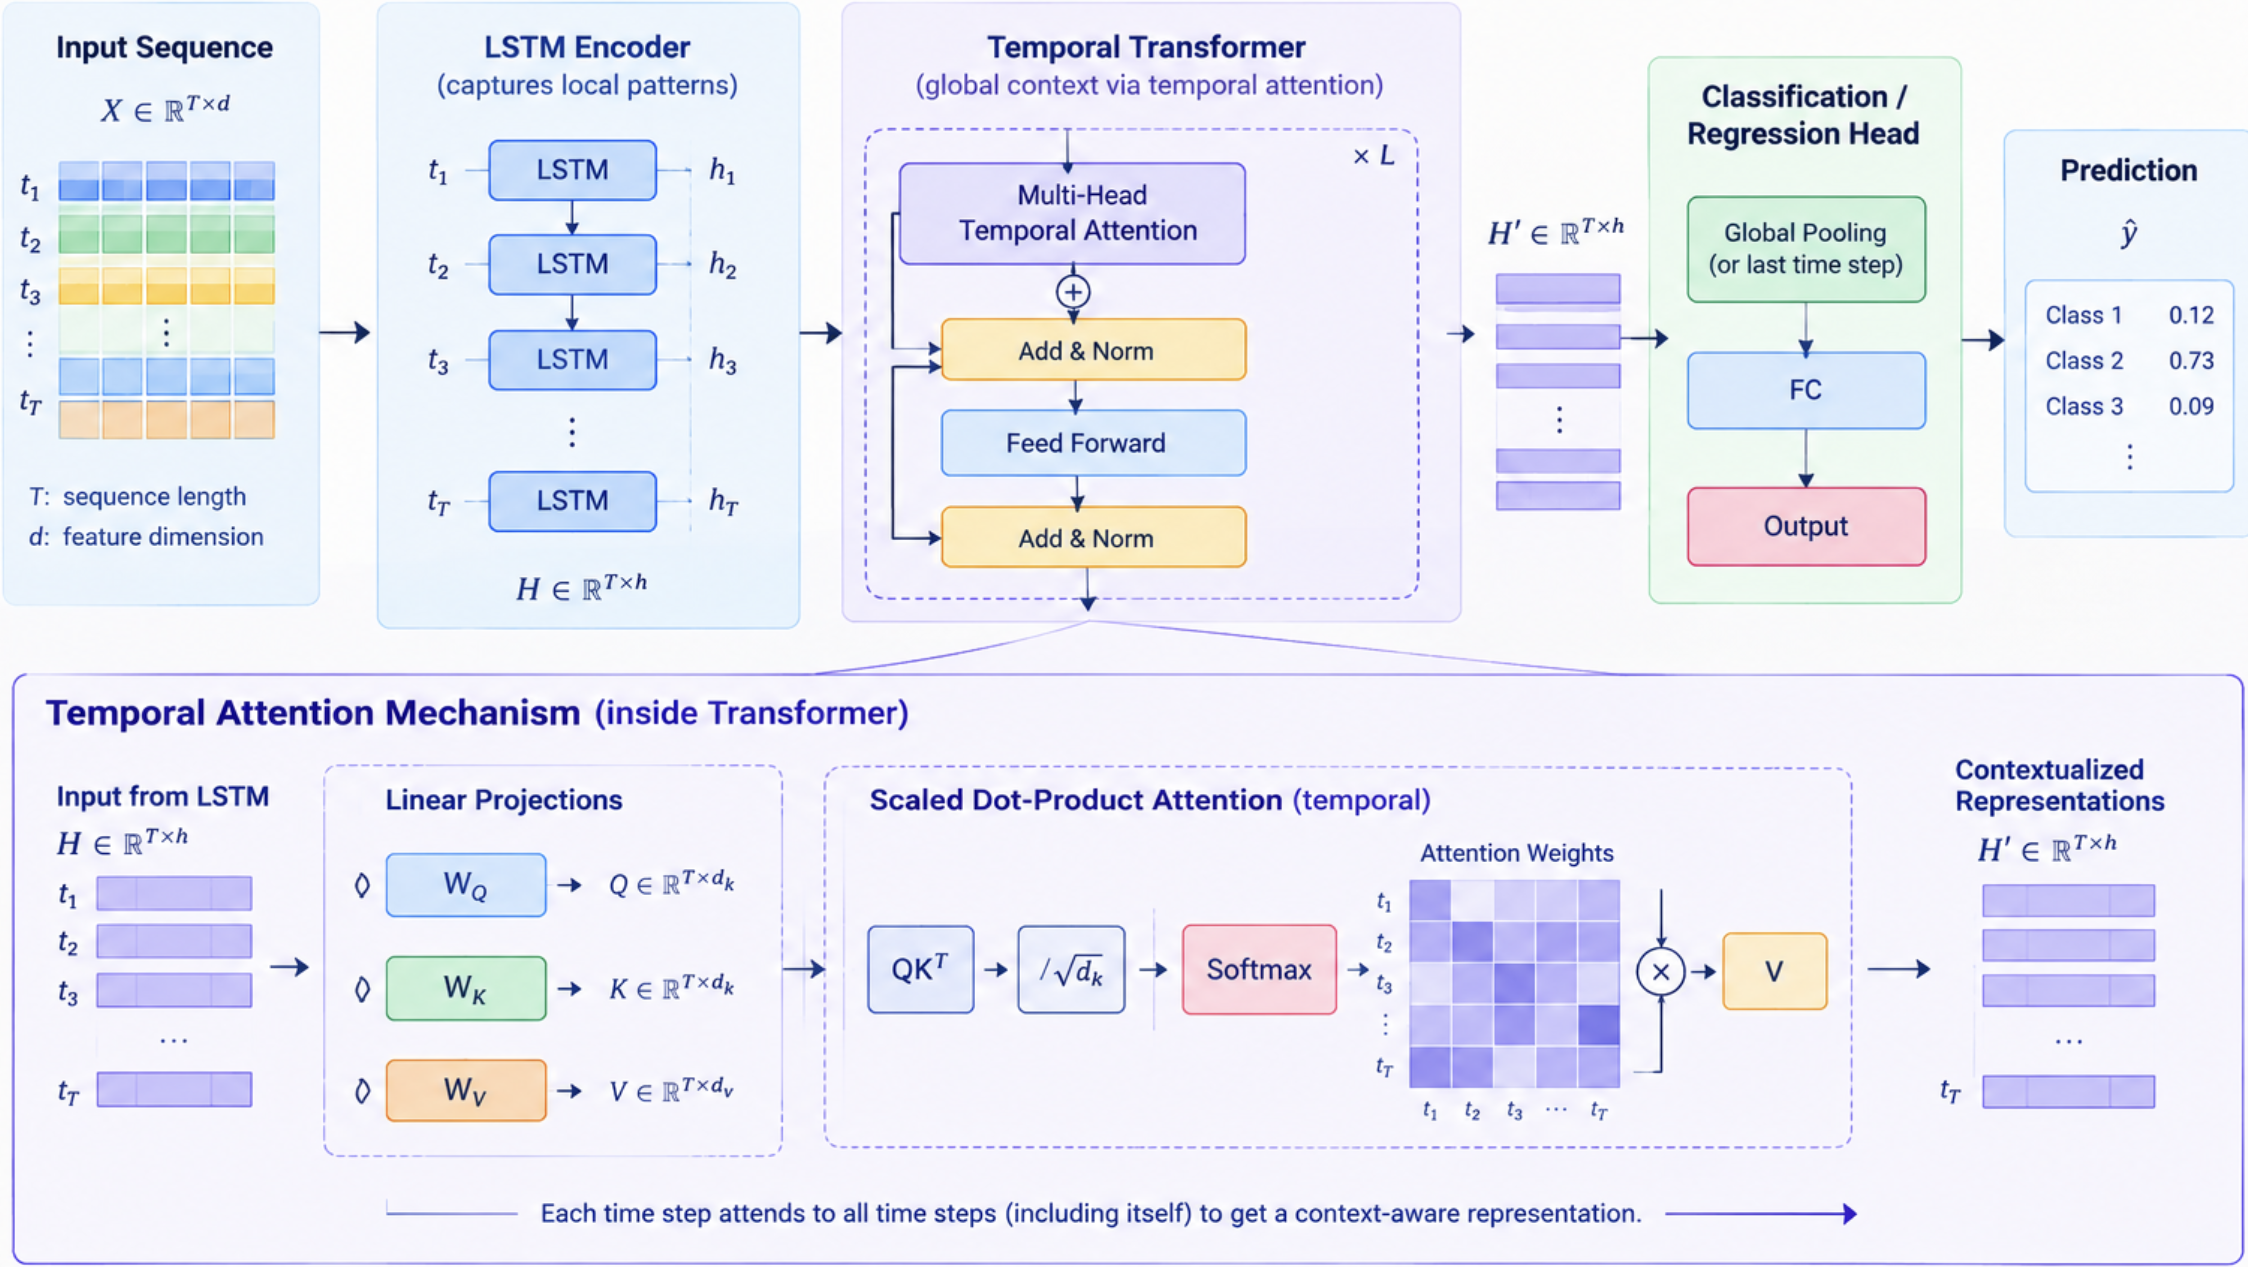
\includegraphics[width=\textwidth]{images/architecture.png}
	\caption{\acs{LSTM}-Transformer Architecture}
	\label{fig:lstm-transformer}
\end{figure}

\subsection{Temporal Encoding (\acs{LSTM})} \label{subsec:temporal-encoding-lstm}
\subsection{Context Layer (Cross-Sectional Transformer)} \label{subsec:context-layer-transformer}
\subsection{Hybrid Loss Function} \label{subsec:hybrid-loss-function}

\section{Hyperparameter Optimization} \label{sec:hyperparameter-optimization}
\section{Training Procedure} \label{sec:training-procedure}
\clearpage

\startfooter{Specialized Project: HK261-DAGD1-041\\
    Empirical Results
}

\part{Empirical Results}
\label{results}

\section{Descriptive Statistics and Data Diagnostics}

\subsection{Dataset Characteristics}

\subsection{Target and Feature Diagnostics}

\section{Predictive Performance}

\subsection{\acs{IC}/\acs{ICIR}}

\subsection{Decile Portfolio Monotonicity}

\subsection{Kendall's Tau Analysis}

\section{Statistical Diagnostics}

\subsection{Statistical Significance}

\subsection{Multiple-Testing and Overfitting Diagnostics}

\section{Ablation Results}

\subsection{Model Architecture Ablation}

\subsection{Loss Function Ablation}

\subsection{Stock ID Embedding Ablation}

% \section{Portfolio Performance}

% \subsection{Portfolio Construction}

% \subsection{Pre-Cost Performance}

% \subsection{Post-Cost Performance}

% \section{Robustness and Stability Analysis}

% \subsection{Walk-Forward Stability}

% \subsection{Regime Stability}

% \subsection{Sensitivity Analysis}

\section{Explainability and Regime-Conditioned Analysis}

\subsection{Integrated Gradients Attribution}

\subsection{Feature Importance Across Volatility Regimes}

\subsection{Surrogate Model Fidelity}

\subsection{Interpretation of Model Behavior}
\clearpage

\part{Limitations and Discussion}
\clearpage
\part{Conclusion}

\startfooter{Specialized Project: HK261-DAGD1-041\\
	Nested Walk-Forward Cross-Validation}

\renewcommand{\addappheadtotoc}{%
	\phantomsection
	\addcontentsline{toc}{part}{\appendixtocname}%
}

\begin{appendices}
	\section{Nested Walk-Forward Cross-Validation}
\label{app:nwfcv}

Deep learning architectures, such as \acf{LSTM} networks, Temporal Convolutional Networks (TCNs), and Spatio-Temporal Graph Neural Networks (ST-GNNs), are increasingly applied to complex panel datasets. These datasets, common in quantitative finance, econometrics, epidemiology, and meteorology, consist of multiple entities (the cross-section) observed over multiple time steps.

\medskip

When training these high-capacity models, practitioners face two primary forms of data leakage:
\begin{enumerate}
	\item \textbf{Temporal leakage (look-ahead bias):} utilizing future information to predict past or present states.
	\item \textbf{Cross-sectional leakage:} normalizing or scaling data using aggregate statistics that include testing periods across different entities.
\end{enumerate}

To rigorously evaluate generalization, the validation scheme must respect the strict arrow of time while accommodating the cross-sectional dimension. The Nested Walk-Forward Cross-Sectional Validation method is designed for this purpose, providing a conservative and realistic estimate of how a model will perform in a sequential production environment. The approach combines rolling-origin evaluation for time-series forecasting \citep{hyndman2021forecasting} with the principle that hyperparameter selection and final performance estimation must be performed on separate data \citep{cawley2010overfitting}.

\subsection{Theoretical Foundation}

\paragraph{Standard Validation versus Temporal Realities}
In standard machine learning, $k$-fold cross-validation randomly partitions the dataset into $k$ subsets, iteratively using $k-1$ folds for training and one for testing. For panel data, random shuffling destroys temporal autocorrelation and allows the model to access information from future periods. Even grouped $k$-fold validation, which keeps observations from the same entity together, does not respect the temporal ordering of the data and therefore cannot account for regime shifts or non-stationarity over time. In financial applications, these violations are especially consequential because overlapping forward-looking labels and low signal-to-noise ratios can produce misleadingly strong in-sample results \citep{lopezdeprado2018advances}.

\begin{table}[H]
	\footnotesize
	\centering
	\caption{\small Comparison of Validation Methods for Panel Data}
	\label{tab:comparison}
	\begin{tabular}{@{}lcccc@{}}
		\toprule
		\textbf{Method}              & \textbf{Time-respected?} & \textbf{Unbiased HP tuning?} & \textbf{Cross-section intact?} & \textbf{Cost} \\
		\midrule
		Standard $k$-fold            & No                       & No                           & Broken                         & Low           \\
		Grouped $k$-fold             & No                       & No                           & Intact                         & Low           \\
		Simple walk-forward          & Yes                      & No                           & Intact                         & Medium        \\
		\textbf{Nested walk-forward} & \textbf{Yes}             & \textbf{Yes}                 & \textbf{Intact}                & \textbf{High} \\
		\bottomrule
	\end{tabular}
\end{table}

\paragraph{Walk-Forward Validation}
Walk-forward validation, also known as rolling-origin evaluation or backtesting, ensures that the training set strictly precedes the validation or test set chronologically \citep{pardo2008evaluation}. Let the dataset be indexed by time $t \in \{1,2,\dots,T\}$. A walk-forward setup evaluates the model at time $t$ using only data from $1$ to $t-1$ (expanding window) or from $t-w$ to $t-1$ (rolling window of size $w$). This structure emulates the repeated retraining and prediction process that would occur in live deployment.

\paragraph{The Necessity of the Nested Approach}
Deep learning models possess numerous hyperparameters, including learning rate, dropout rate, number of layers, embedding dimensions, and window lengths. If a simple walk-forward procedure uses the validation period both to select hyperparameters and to report final performance, the resulting metrics are optimistically biased. This phenomenon, known as \textit{overfitting to the validation set}, arises because repeated model selection on the same validation data effectively incorporates information about that data into the modeling pipeline \citep{cawley2010overfitting}.

\medskip

A nested approach addresses this problem by strictly separating hyperparameter selection from out-of-sample performance estimation through two distinct, temporally ordered loops:

\begin{itemize}
	\item \textbf{Inner loop (hyperparameter optimization):} This loop operates entirely within the training window of the current outer step. It performs its own chronological walk-forward validation across multiple historical folds. For a given hyperparameter configuration, the model is trained and evaluated sequentially, and the average validation performance determines the configuration’s fitness. Because every inner validation set precedes the corresponding outer test set, the selected hyperparameters contain no look-ahead information about the subsequent out-of-sample period \citep{cawley2010overfitting, kodeli2022time}.

	\item \textbf{Outer loop (unbiased evaluation):} The outer loop simulates sequential deployment over time. Once the inner loop identifies the best hyperparameter configuration, a new model is trained using that configuration on all historical data available up to the outer test date. The model is then evaluated on strictly future observations. Advancing the outer window through time produces a sequence of genuinely out-of-sample predictions, whose aggregation provides a realistic estimate of end-to-end pipeline performance \citep{pardo2008evaluation, hyndman2021forecasting}.
\end{itemize}

\begin{figure}[H]
	\centering
	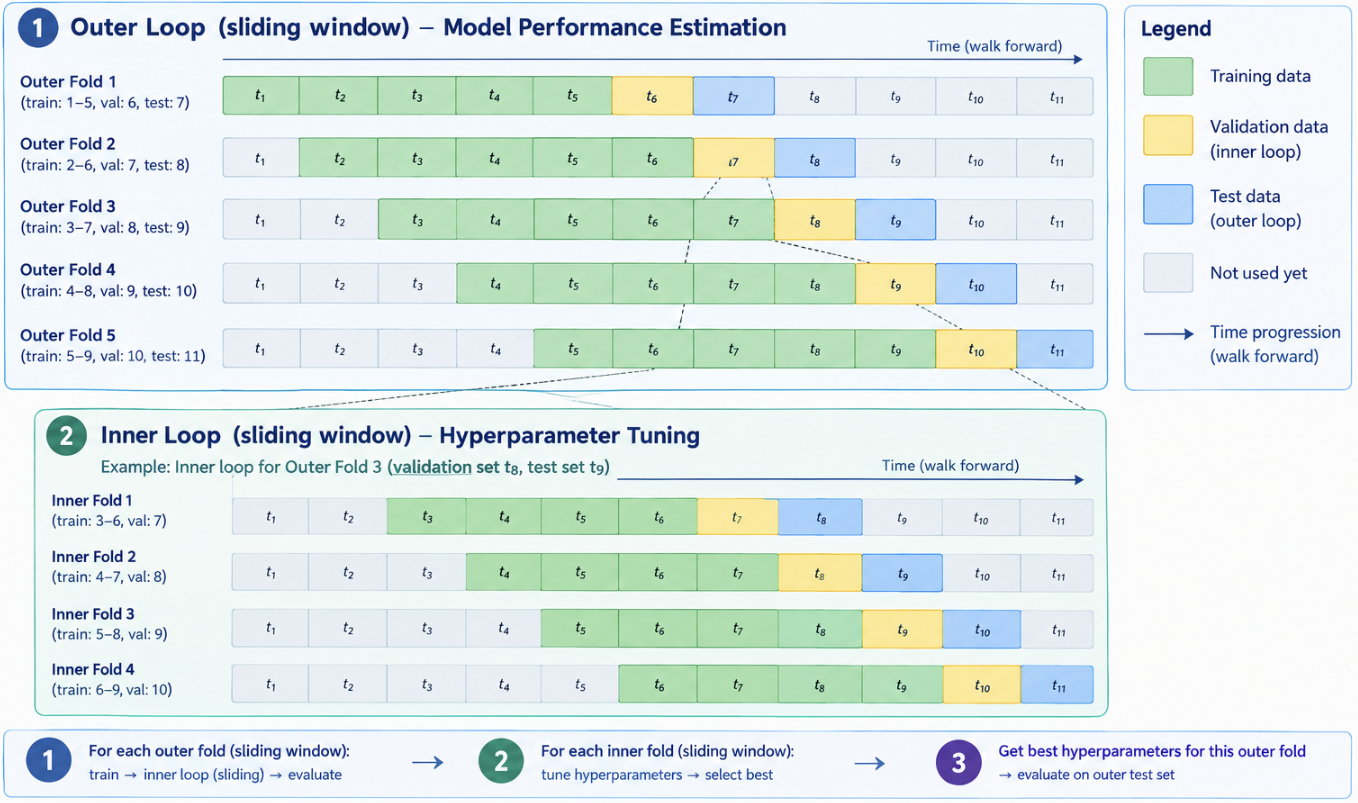
\includegraphics[width=\textwidth]{images/NWFCV.png}
	\caption{Walk-Forward Cross-Sectional Validation Visualization}
	\label{fig:NWFCV}
\end{figure}

\subsubsection*{Leakage Control for Overlapping Financial Labels}
When the target variable is a multi-period forward return or another overlapping label, temporal separation of training and test dates alone may not eliminate leakage. In that case, training observations whose label horizons overlap the validation or test interval should be removed through purging, and an embargo period may be added after the training window to attenuate serial dependence across adjacent periods \citep{lopezdeprado2018advances}. These safeguards should be applied consistently in both the inner and outer loops. A nested walk-forward implementation of this type has been used in cross-sectional equity-return prediction, where an outer walk-forward loop evaluates performance year by year while an inner leave-one-year-out procedure selects the regularization parameter using only prior-year data \citep{kodeli2022time}.

\subsection{Formal Specification}

\subsubsection{Mathematical Formulation}

\begin{algorithm}[H]
	\captionsetup{font=small}
	\caption{Nested Walk-Forward Cross-Sectional Validation Pseudocode}
	\begin{algorithmic}[1]\footnotesize
		\Require Dataset $\mathcal{D}$ sorted by time $t$, hyperparameter search space $H$, initial training window $W_{\mathrm{init}}$, step size $S$.
		\State $E_{\mathrm{OOS}} \gets []$ \Comment{Out-of-sample errors}
		\For{$T_{\mathrm{test}} = W_{\mathrm{init}}$ \textbf{to} $T$ \textbf{step} $S$}
		\State $\mathcal{D}_{\mathrm{outer\_train}} \gets \mathcal{D}[:T_{\mathrm{test}}-1]$
		\State $\mathcal{D}_{\mathrm{outer\_test}} \gets \mathcal{D}[T_{\mathrm{test}}:T_{\mathrm{test}}+S-1]$
		\State $best\_h \gets \mathrm{null}$, $min\_val\_loss \gets \infty$

		\For{$h \in H$} \Comment{Inner loop: hyperparameter tuning}
		\State $val\_loss \gets 0$
		\State Define chronological inner validation splits within $\mathcal{D}_{\mathrm{outer\_train}}$
		\For{each inner split $(\mathcal{D}_{\mathrm{inner\_train}}, \mathcal{D}_{\mathrm{inner\_val}})$}
		\State $\theta \gets \mathrm{InitializeWeights}()$
		\State $\theta \gets \mathrm{TrainDeepModel}(\mathcal{D}_{\mathrm{inner\_train}}, \theta, h)$
		\State $val\_loss \gets val\_loss + \mathrm{EvaluateCrossSection}(\mathcal{D}_{\mathrm{inner\_val}}, \theta)$
		\EndFor
		\State $val\_loss \gets val\_loss / \mathrm{number\_of\_inner\_splits}$
		\If{$val\_loss < min\_val\_loss$}
		\State $min\_val\_loss \gets val\_loss$
		\State $best\_h \gets h$
		\EndIf
		\EndFor

		\State \Comment{Outer loop: final training and evaluation}
		\State $\theta_{\mathrm{final}} \gets \mathrm{InitializeWeights}()$
		\State $\theta_{\mathrm{final}} \gets \mathrm{TrainDeepModel}(\mathcal{D}_{\mathrm{outer\_train}}, \theta_{\mathrm{final}}, best\_h)$
		\State $err \gets \mathrm{EvaluateCrossSection}(\mathcal{D}_{\mathrm{outer\_test}}, \theta_{\mathrm{final}})$
		\State $E_{\mathrm{OOS}}.\mathrm{append}(err)$
		\EndFor
		\State \Return $\mathrm{Mean}(E_{\mathrm{OOS}})$
	\end{algorithmic}
\end{algorithm}
Consider a panel dataset $\mathcal{D} = \{(\mathbf{x}_{i,t}, y_{i,t})\}$, where $i \in \{1,\dots,N\}$ denotes the cross-sectional entity and $t \in \{1,\dots,T\}$ denotes the time step. Here, $\mathbf{x}_{i,t} \in \mathbb{R}^d$ is the feature vector and $y_{i,t}$ is the target variable.

\medskip

Let $H$ be the set of candidate hyperparameter configurations, and let the outer test dates be $T_{\mathrm{test}}^{(1)}, T_{\mathrm{test}}^{(2)}, \dots, T_{\mathrm{test}}^{(K)}$.

\medskip

For the $k$-th outer fold at time $T_{\mathrm{test}}^{(k)}$:
\begin{enumerate}[topsep=0pt, itemsep=0pt, parsep=0pt]
	\item \textbf{Outer training window:} The available data are
	      \begin{equation}
		      \mathcal{D}_{\mathrm{train}}^{(k)}
		      =
		      \left\{
		      (\mathbf{x}_{i,t}, y_{i,t})
		      \mid
		      t < T_{\mathrm{test}}^{(k)}
		      \right\}.
	      \end{equation}

	\item \textbf{Inner loop (hyperparameter optimization):}
	      Split $\mathcal{D}_{\mathrm{train}}^{(k)}$ into further chronological sub-windows. Let the inner test dates be $\tau^{(1)}, \tau^{(2)}, \dots, \tau^{(J)}$, where $\tau^{(j)} < T_{\mathrm{test}}^{(k)}$. For each hyperparameter configuration $h \in H$,
	      \begin{equation}
		      \mathrm{Score}(h)
		      =
		      \dfrac{1}{J}
		      \sum_{j=1}^{J}
		      \mathcal{L}
		      \left(
		      \mathcal{M}_h
		      \left(
		      \mathcal{D}_{\mathrm{train},\tau^{(j)}}
		      \right),
		      \mathcal{D}_{\mathrm{test},\tau^{(j)}}
		      \right),
		      \label{eq:inner-score}
	      \end{equation}
	      where $\mathcal{M}_h$ is the model trained with hyperparameters $h$ and $\mathcal{L}$ is a cross-sectional loss, such as mean squared error or cross-entropy computed across all $N$ entities at time $\tau^{(j)}$. The selected configuration is
	      \begin{equation}
		      h_{\mathrm{opt}}^{(k)}
		      =
		      \arg\min_{h \in H}
		      \mathrm{Score}(h).
	      \end{equation}

	\item \textbf{Outer loop (evaluation):}
	      The final model is trained on the full outer training window using the selected configuration:
	      \begin{equation}
		      \mathcal{M}_{\mathrm{final}}^{(k)}
		      =
		      \mathrm{Train}
		      \left(
		      \mathcal{D}_{\mathrm{train}}^{(k)},
		      h_{\mathrm{opt}}^{(k)}
		      \right).
		      \label{eq:final-model}
	      \end{equation}
	      Its out-of-sample performance is evaluated on the cross-section at $T_{\mathrm{test}}^{(k)}$:
	      \begin{equation}
		      \mathrm{Error}^{(k)}
		      =
		      \mathcal{L}
		      \left(
		      \mathcal{M}_{\mathrm{final}}^{(k)},
		      \left\{
		      (\mathbf{x}_{i,T_{\mathrm{test}}^{(k)}},
		      y_{i,T_{\mathrm{test}}^{(k)}})
		      \right\}_{i=1}^{N}
		      \right).
		      \label{eq:outer-error}
	      \end{equation}
\end{enumerate}

The final estimate of generalization performance is obtained by aggregating $\mathrm{Error}^{(k)}$ across all outer folds. Because each evaluation uses a model trained and tuned exclusively on earlier data, the resulting metric reflects the expected performance of the complete modeling pipeline under sequential deployment \citep{hyndman2021forecasting, pardo2008evaluation}.

\subsubsection{Quantitative Finance Mathematical Formulation}
To adapt Nested Walk-Forward Cross-subSectional Validation to systematic trading and quantitative portfolio construction, market microstructure dynamics and risk constraints are explicitly formalized below.

\paragraph{Cross-Sectional Alpha Optimization}
Let $\mathbf{r}_{t+1} \in \mathbb{R}^N$ denote the forward return vector for an asset universe $\mathcal{U} = \{1, \dots, N\}$ at timestamp $t$. The neural network $f_\theta: \mathbb{R}^{N \times d} \to \mathbb{R}^N$ maps asset features $\mathbf{X}_t$ to predicted alpha scores $\mathbf{\hat{r}}_{t+1} = f_\theta(\mathbf{X}_t)$.

\begin{definition}[Cross-Sectional Z-Score Operator]
	For any vector $\mathbf{v} \in \mathbb{R}^N$, the cross-sectional normalization operator $\mathbf{Z}: \mathbb{R}^N \to \mathbb{R}^N$ is defined as:
	\begin{equation}
		\mathbf{Z}(\mathbf{v}) = \dfrac{v - \bar{v}}{\sigma_{\mathbf{v}}}, \quad \bar{v} = \dfrac{1}{N}\sum_{i=1}^N v_i, \quad \sigma_{\mathbf{v}} = \sqrt{\dfrac{1}{N}\sum_{i=1}^N (v_i - \bar{v})^2}
	\end{equation}
\end{definition}

\begin{definition}[Differentiable Information Coefficient Loss]
	The network optimizes the cross-sectional Pearson correlation (Information Coefficient) between predicted rankings and realized forward returns:
	\begin{equation}
		\mathcal{L}_{\text{IC}}(\theta; \mathbf{X}_t, \mathbf{r}_{t+1}) = - \dfrac{1}{N} \mathbf{Z}\left(f_\theta(\mathbf{X}_t)\right)^\top \mathbf{Z}\left(\mathbf{r}_{t+1}\right)
	\end{equation}
\end{definition}

\paragraph{Purging and Embargo Operators}
For an $h$-period forward return target $y_{i,t} = \displaystyle\prod_{k=1}^h (1 + r_{i,t+k}) - 1$, overlapping target horizons introduce non-zero temporal covariance across model residuals.
\begin{definition}[Information Leakage Sets]
	Given an inner validation set $\mathcal{T}_{\text{val}} = [t_{\text{v,start}}, t_{\text{v,end}}]$ and an embargo horizon $e \ge h$:
	\begin{align}
		\text{Purged Set: } \mathcal{P}(\mathcal{T}_{\text{val}})     & = \{ t \mid t_{\text{v,start}} - h + 1 \le t < t_{\text{v,start}} \} \\
		\text{Embargo Set: } \mathcal{E}(\mathcal{T}_{\text{val}}, e) & = \{ t \mid t_{\text{v,end}} < t \le t_{\text{v,end}} + e \}
	\end{align}
	The strictly admissible training set $\mathcal{T}_{\text{train}}^{\text{admissible}}$ is given by:
	\begin{equation}
		\mathcal{T}_{\text{train}}^{\text{admissible}} = \mathcal{T}_{\text{hist}} \setminus \left( \mathcal{T}_{\text{val}} \cup \mathcal{P}(\mathcal{T}_{\text{val}}) \cup \mathcal{E}(\mathcal{T}_{\text{val}}, e) \right)
	\end{equation}
\end{definition}

\paragraph{Inner Loop Hyperparameter Selection Objective}
To avoid validation overfit under a low signal-to-noise ratio ($\text{SNR} \ll 1$), the inner-loop hyperparameter fitness function $g(h)$ evaluates risk-adjusted portfolio performance across $J$ inner folds:
\begin{equation}
	h_{\text{opt}}^{(k)} = \arg\max_{h \in H} \dfrac{1}{J} \sum_{j=1}^J \left[ \dfrac{\mu_{\text{IC}}(h, j)}{\sigma_{\text{IC}}(h, j) + \epsilon} + \lambda \cdot \text{Sharpe}\left( \mathbf{w}_t^*(f_{\theta_{h,j}}) \right) \right]
\end{equation}
where portfolio weights $\mathbf{w}_t^* \in \mathbb{R}^N$ solve the mean-variance transaction-cost constrained problem:
\begin{equation}
	\mathbf{w}_t^*(\mathbf{\hat{r}}_{t+1}) = \arg\max_{\mathbf{w} \in \mathcal{W}} \left( \mathbf{w}^\top \mathbf{\hat{r}}_{t+1} - \dfrac{\gamma}{2} \mathbf{w}^\top \boldsymbol{\Sigma}_t \mathbf{w} - \kappa \|\mathbf{w} - \mathbf{w}_{t-1}\|_1 \right)
\end{equation}

\paragraph{Regime Drift Regularization via Proximal Updates}
To reduce computational burden while adapting to market regime changes, outer model weights $\theta^{(k)}$ undergo proximal updating from step $k-1$:
\begin{equation}
	\theta^{(k)} = \arg\min_{\theta} \left( \sum_{t \in \mathcal{D}_{\text{outer}}^{(k)}} \mathcal{L}_{\text{IC}}(\theta; \mathbf{X}_t, \mathbf{r}_{t+1}) + \dfrac{\mu}{2} \left\| \theta - \theta^{(k-1)} \right\|_{\mathbf{F}}^2 \right)
\end{equation}
where $\|\mathbf{v}\|_{\mathbf{F}}^2 = \mathbf{v}^\top \mathbf{F} \mathbf{v}$, and $\mathbf{F} = \mathbb{E}\left[ \nabla_\theta \mathcal{L} \left(\nabla_\theta \mathcal{L}\right)^\top \right]$ is the diagonal Fisher Information Matrix.

\subsection{Conclusion}
The Nested Walk-Forward Cross-Sectional Validation method is a rigorous framework for developing deep learning models on time-series panel data, where temporal leakage can invalidate performance estimates. By structurally separating hyperparameter search in the inner loop from temporal out-of-sample evaluation in the outer loop, and by evaluating errors across the cross-sectional dimension, it provides robust and realistic performance metrics \citep{cawley2010overfitting, pardo2008evaluation}. Although computationally expensive, the procedure is particularly valuable in applications such as algorithmic trading, macroeconomic forecasting, epidemiology, and personalized medicine, where deployment decisions depend on reliable estimates of future performance \citep{lopezdeprado2018advances, hyndman2021forecasting}.
	\startfooter{Specialized Project: HK261-DAGD1-041\\
             Performance Framework and Alpha Metrics
}
\section{Performance Framework and Alpha Metrics}
\subsection{Information Efficiency Metrics}
\subsubsection*{\acf{IC}}
\subsubsection*{\acf{ICIR}}
\end{appendices}
\newpage
\bibliographystyle{alpha}
\bibliography{references}
\end{document}